\chapter{人工データ実験}
\section{シミュレーション}
ニューロン集団のカルシウムイメージングデータをシミュレーションによって作り,解析手法を評価する.
シミュレーションには1)ニューロンのネットワーク構造を作成し,2)スパイクのシミュレーションを行い,3)蛍光強度の観測データに変換する.
\subsection{ネットワーク構造}
ニューロンのネットワーク構造にはsmall world network\cite{}を用いる.
Small world networkはノード数,張り替え確率,初期次数を決めることによってネットワークを作成するアルゴリズムである.
初期次数は,ニューロンが平均何このニューロンとコネクションを持つかという変数である.
張り替え確率は,初期次数によって作成された規則的なグラフのエッジをこの確率でランダムに張り替える.
そのため,エッジのうち何割が遠くのニューロンとつながっているかを表す変数である.

ここでいうコネクティビティとは,synaptic connectivityである.
脳のコネクティビティには3種類あり,synaptic connectivityとanatomical connectivityとfunctional connectivityである.
Synaptic connetivityはニューロンがシナプスを形成してつながっている状態のことである.

実際のニューロンをsmall world networkによって表すために,初期次数と張り替え確率を実データから決める.
今回はこの値はニューロンのコネクションの割合と相互のコネクションの割合から決める.
興奮性ニューロン同士の6.7\%であり,そのうち双方向のコネクションの割合は24\%である\cite{}.
成熟したマウスの抑制性ニューロンと興奮性ニューロンのコネクションの割合は不明だが,興奮性ニューロンから抑制性ニューロンへのコネクティビティと抑制性ニューロンから興奮性ニューロンへのコネクティビティはどちらも78\%であった\cite{Holmgren2003}.
成熟したマウスではより少ないと思われるが,データが見つからなかったため,40\%とした.
相互のコネクションの割合がランダムにエッジを作るよりも高いのは,近いニューロンにコネクションが作られやすいからだと考えられる.
これらのデータを実現するように初期次数と張り替え確率を調整した.
また,抑制性ニューロン同士のコネクティビティは分からないため,興奮性と同じにしている.
\subsection{スパイクシミュレーション}
We use spiking model proposed by Izhikevichモデル~\cite{Izhikevich2003}.
This model is based on Hodgkin-Huxley model with computational efficiency.
There are 4 parameters in thid model which characterize neuron types.
We used regular spiking neurons for excitatory neurons and fast spiking neurons for inhibitory neurons.
The parameters we used is shown in \Tabref{tab:parameter1} where $r_e$ and $r_i$ are random variables following a uniform distribution from 0 to 1.

\begin{table}[htb]
  \center
  \begin{tabular}{|c|cccc|} \hline
    neuron type & a & b & c & d \\ \hline
    excitatory neuron & 0.02 & 0.2 & $-65 + 15 r_e^2$ & $8 - 6r_e^2$ \\
    inhibitory neuron & $0.02 + 0.08r_i$ & $0.25 - 0.05 r_i$ & -65 & 2 \\ \hline
  \end{tabular}
  \caption{Parameters used in Izhikevich model}
  \label{tab:parameter1}
\end{table}

We need to specify synaptic transmissions between neurons.
It can be written by adjacency matrix.
The $(i,j)$-element of the adjacency matrix equals to how much voltage will be transmitted from neuron $j$ to neuron $i$ when neuron $j$ is fired.
The columns of excitatory neurons and inhibitory neurons are random variables following a uniform distribution from 0 to 0.5 and a uniform distribution from -2 to 0, respectively.

We simulated for a network of 800 excitatory neurons and 200 inhibitory neurons.
Every neuron has random thalamic input from outside the network in every 1ms.
Thalamic input for excitatory neurons and inhibitory neurons follow a gaussian distribution with mean 0 and variance 5 and a gaussian distribution with mean 0 and variance 2, respectively.
We need to evaluate NMF by the ability of detecting neural ensembles which is activated in specific time.
The number of neurons in each ensemble follows a uniform distribution from 50 to 200.
We changed neural ensembles every 10s.
In that time period, neurons in ensemble have stronger thalamic input raised by 1 and 0.4 for excitatory and inhibitory neurons, respectively.
Total time of simulation is 470s.
The first 10s is not used for the simulation stability.

\subsection{Calcium imaging model}
We calculate calcium concentration in a neuron from simulated spikes by following model proposed by Vogelstein~\cite{Vogelstein2009}:
\begin{equation}
  [Ca^{2+}]_{i,t} - [Ca^{2+}]_{i,t-1} = - \frac{\Delta}{\tau}([Ca^{2+}]_{t-1} - [Ca^{2+}]_b) + An_{i,t} + \sigma_c \sqrt{\Delta} \epsilon_{i,t},
  \label{eq:calcium}
\end{equation}
where $[Ca^{2+}]_{i,t}$ is calcium concentration of neuron $i$ at time $t$, $[Ca^{2+}]_b$ is calcium concentration baseline, $\Delta$ is time step size, $\tau$ is decay time constant, $A$ is rise in $[Ca^{2+}]$ after spike, $n_{i,t}$ is spike of 0 or 1, $\sigma_c$ is variance of noise, $\epsilon_{i,t}$ is noise which follows normal gaussian distribution.
We do not take saturation into account because our data seems to be not having saturation.

Then, we convert the calcium concentration $[Ca^{2+}]_{i,t}$ to imaging intensity $F_{i,t}$ by equation from Vogelstein~\cite{Vogelstein2009}:
\begin{equation}
  F_{i,t} = \alpha[Ca^{2+}]_t + \beta + \sigma_F \epsilon_{i,t},
  \label{eq:intensity}
\end{equation}
where $\alpha$ is the scale of imaging intensity, $\beta$ is offset, $sigma_F$ is variance of noise and $\epsilon_{i,t}$ is noise which follows normal gaussian distribution.

Finally, we take sum of intensity every 125ms since our data is sampled at 8Hz:
\begin{equation}
  x_{i,t'} = \sum_{t=1}^{125} F_{i,t}.
  \label{eq:observation}
\end{equation}

Parameters we used is shown in \Tabref{tab:parameter2}.
\begin{table}[htb]
  \center
  \begin{tabular}{|cccccccc|} \hline
    $[Ca^{2+}]_b$ & $\Delta$ & $\tau$ & $A$ & $\sigma_c$ & $\alpha$ & $\beta$ & $\sigma_F$ \\ \hline
    0.1 & 0.001 & 0.5 & 5.0 & 1.0 & 1.0 & 0 & 1.0 \\ \hline
  \end{tabular}
  \caption{Parameters used in Vogelstein model}
  \label{tab:parameter2}
\end{table}

\section{結果}
人工データは4種類作成した.
\begin{enumerate}
  \item ニューロンは1つのグループに必ず所属し,近いニューロン同士がグループとなっている
  \item ニューロンは1つのグループに必ず所属し,グループは近さに関係なくランダムに形成される
  \item ニューロンは1つか2つのグループに必ず所属し,同じニューロンが所属しているグループ同士の活動は被らない
\end{enumerate}

\subsection{手法の比較}
Euclidean NMF,logistic regression,glassoの性能の比較を行った.
2のタイプについて100種類のデータを生成し,ニューロン同士が同じグループにあるか否かの行列のF1 scoreを比較した.
\begin{figure}[htbp]
    \begin{center}
        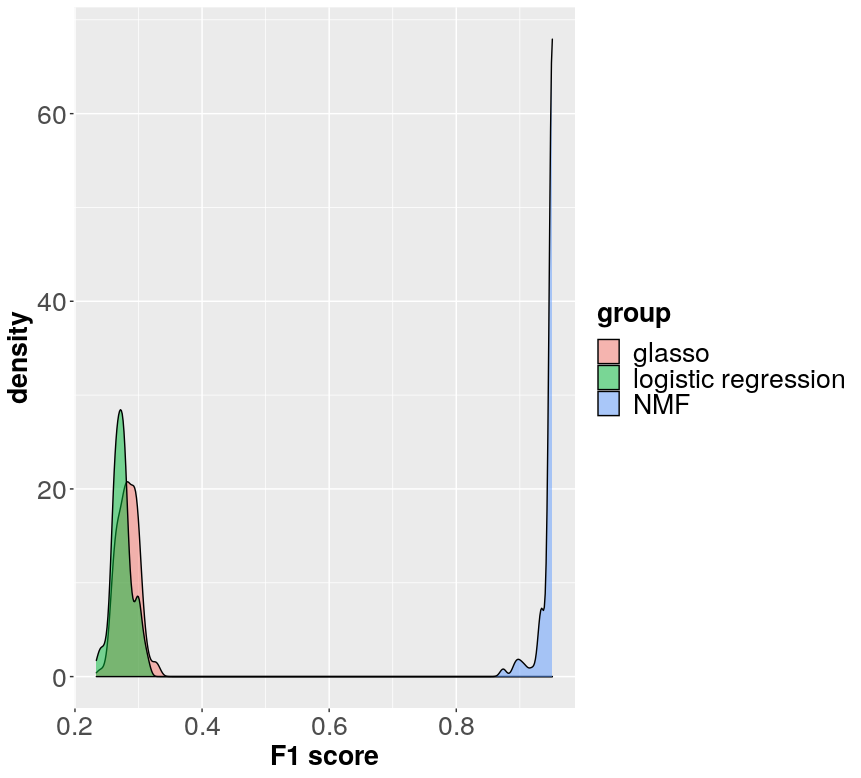
\includegraphics[width=0.5\linewidth]{compare3}
        \caption{NMF,logistic regression,glassoのF1 scoreの密度分布}
        \label{fig:compare3}
    \end{center}
\end{figure}
\Figref{fig:compare3}より,glassoとlogistic regressionの精度は低いことがわかる.
3つの手法のうちNMFがカルシウムイメージングデータを扱うのに適していると考えられる.

\subsection{推定へのネットワーク構造の影響}
グループ推定へのネットワーク構造の影響を調べるために,1と2のネットワーク構造とグループについて100種類のデータを生成し,NMFの推定精度の比較を行った.
人工データは,近いニューロンほどつながりやすい性質をもつので,1の人工データの方がニューロン同士が同期して活動しやすいと思われる.
ここで,2つのニューロンが同期するとは,一方のニューロンが発火してからごく短い間にもう一方のニューロンが発火する状態が続くことである.
実験結果を\Figref{fig:same-exc}~\ref{fig:diff-inh}に示す.
\begin{figure}[htbp]
    \begin{center}
        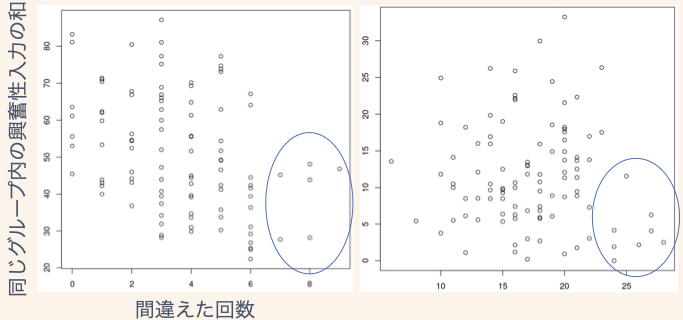
\includegraphics[width=\linewidth]{same-exc}
        \caption{データ1と2について,ニューロンごとの間違えた回数と同じグループからの興奮性入力の和の関係}
        \label{fig:same-exc}
    \end{center}
\end{figure}
\begin{figure}[htbp]
    \begin{center}
      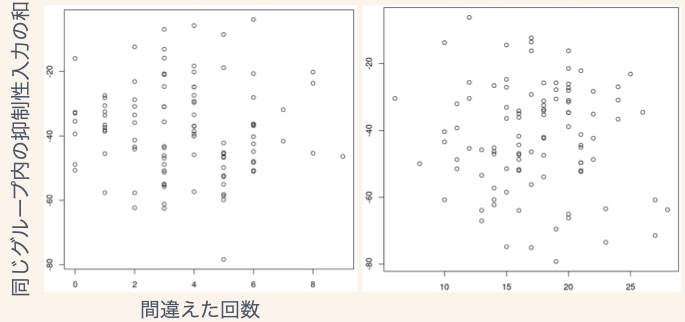
\includegraphics[width=\linewidth]{same-inh}
        \caption{データ1と2について,ニューロンごとの間違えた回数と同じグループからの抑制性入力の和の関係}
        \label{fig:same-inh}
    \end{center}
\end{figure}
\begin{figure}[htbp]
    \begin{center}
        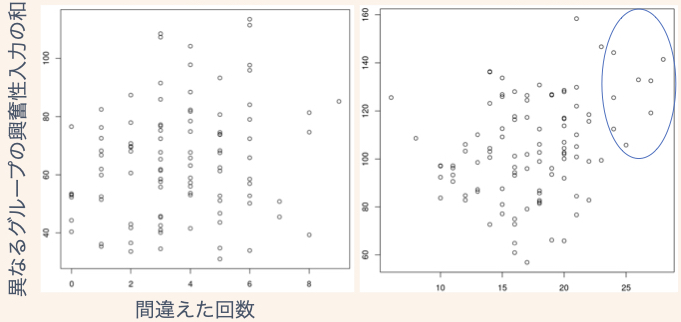
\includegraphics[width=\linewidth]{diff-exc}
        \caption{データ1と2について,ニューロンごとの間違えた回数と異なるグループからの興奮性入力の和の関係}
        \label{fig:diff-exc}
    \end{center}
\end{figure}
\begin{figure}[htbp]
    \begin{center}
        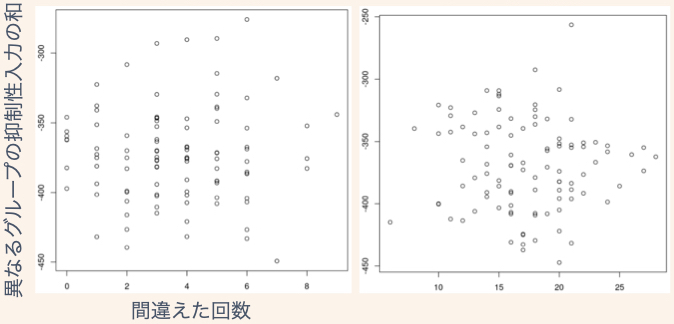
\includegraphics[width=\linewidth]{diff-inh}
        \caption{データ1と2について,ニューロンごとの間違えた回数と異なるグループからの興奮性入力の和の関係}
        \label{fig:diff-inh}
    \end{center}
\end{figure}
\Figref{fig:same-inh},\Figref{fig:diff-inh}より,抑制性の入力は間違える回数には影響しないと思われる.
\Figref{fig:same-exc}より,同じグループからの興奮性入力が小さいと間違えやすいと言える.
\Figref{fig:diff-exc}より,データ2で間違える回数が多かったニューロンは異なるグループからの興奮性入力が大きかった.
データ2ではデータ1よりも近いニューロンが異なるグループに所属する割合が多い.
そのため,異なるグループからの興奮性入力と間違える回数の関係が強く出たと思われる.

他にも推定へのネットワーク構造の影響の調査を試みたが,はっきりとした結果は得られなかった.

\subsection{ブートストラップの有用性}
1回NMFした結果とブートストラップした結果のAのF1 scoreを比較

\subsection{Model Averagingの有用性}
基底数変えてModel averageするとよかったよという話
